%%%%%%%%%%%%%%%%%%%%%%%%%%%%%%%%%%%%%%%%%%%%%%%%%%%%%%%%%%%%%%%%%%%%%%%%%%%%%%
%
% Space Warps System Paper
%
%%%%%%%%%%%%%%%%%%%%%%%%%%%%%%%%%%%%%%%%%%%%%%%%%%%%%%%%%%%%%%%%%%%%%%%%%%%%%%

\documentclass[useAMS,usenatbib,a4paper]{mn2e}
%% letterpaper
%% a4paper

\voffset=-0.6in

% Packages:
\input psfig.sty
\usepackage{xspace}
\usepackage{graphicx}
\usepackage{amssymb}
\usepackage{amsmath}

% Macros:
% JOURNALS
\newcommand{\apj}{ApJ}
\newcommand{\apjl}{ApJL}
\newcommand{\apjs}{ApJS}
\newcommand{\mnras}{MNRAS}
\newcommand{\apss}{Ap \& SS}
\newcommand{\aap}{A\&A}
\newcommand{\aj}{AJ}
\newcommand{\prd}{Phys. Rev. D}
\newcommand{\nat}{Nature}
\newcommand{\araa}{ARA\&A}
\newcommand{\jgr}{J. Geophys. Res.}
\newcommand{\pasp}{PASP}

% MISC
\newcommand{\etal}{et~al.~}
\newcommand{\eg}{{\it e.g.\ }}
\newcommand{\ie}{{\it i.e.\ }}
\newcommand{\etc}{{\it etc.\ }}

\newcommand{\be}{\begin{equation}}
\newcommand{\ee}{\end{equation}}
\newcommand{\bea}{\begin{eqnarray}}
\newcommand{\eea}{\end{eqnarray}}


% CROSS-REFERENCING
\def\Sref#1{Section~\ref{#1}\xspace}
\def\Fref#1{Figure~\ref{#1}\xspace}
\def\Tref#1{Table~\ref{#1}\xspace}
\def\Eref#1{Equation~\ref{#1}\xspace}
\def\Aref#1{Appendix~\ref{#1}\xspace}

% UNITS
\newcommand{\kms}{\ifmmode  \,\rm km\,s^{-1} \else $\,\rm km\,s^{-1}  $ \fi }
\newcommand{\kpc}{\ifmmode  {\rm kpc}  \else ${\rm  kpc}$ \fi  }  
\newcommand{\pc}{\ifmmode  {\rm pc}  \else ${\rm pc}$ \fi  }  
\newcommand{\Msun}{\ifmmode {\rm M_{\odot}} \else ${\rm M_{\odot}}$ \fi} 
\newcommand{\Zsun}{\ifmmode {\rm Z_{\odot}} \else ${\rm Z_{\odot}}$ \fi} 
\newcommand{\yr}{\ifmmode yr^{-1} \else $yr^{-1}$ \fi} 
\newcommand{\hMsun}{\ifmmode h^{-1}\,\rm M_{\odot} \else $h^{-1}\,\rm M_{\odot}$ \fi}

% COSMOLOGY
\newcommand{\LCDM}{$\Lambda{\rm CDM}$}
\newcommand{\MS}{Millennium Simulation\xspace}

% LENSING
\def\zd{z_{\rm d}}
\def\zs{z_{\rm s}}
\def\Dd{D_{\rm d}}
\def\Ds{D_{\rm s}}
\def\Dt{D_{\Delta t}}
\def\Dds{D_{\rm ds}}
\def\Sigmacrit{\Sigma_{\rm crit}}
\def\REin{R_{\rm Ein}}
\def\MEin{M_{\rm Ein}}

% SOFTWARE/HARDWARE
\def\sw{{\small\sc Space\,Warps}\xspace}
\def\SW{{\sc Space\,Warps}\xspace}
\def\Talk{{\small\sc Talk}\xspace}
\def\Letters{{\small\sc Letters}\xspace}
\def\Letter{{\small\sc Letter}\xspace}
\def\Dashboard{{\small\sc Dashboard}\xspace}
\def\cfhtls{{\it CFHTLS}\xspace}
\def\python{{\sc python}\xspace}

% TABLES:
\newcommand\nodata{ ~$\cdots$~ }%

% PROBABILITY THEORY
\def\pr{{\rm Pr}}
\def\data{{\mathbf{d}}}
\def\datap{{\mathbf{d}^{\rm p}}}
\def\datai{d_i}
\def\datapi{d^{\rm p}_i}
\def\LENS{{\rm LENS}}
\def\saidLENS{{\rm ``LENS"}}
\def\NOT{{\rm NOT}}
\def\saidNOT{{\rm ``NOT"}}

% AGENT BUREAUCRACY
\def\effort{N_{\rm C}}
\def\experience{N_{\rm T}}
\def\skill{\langle I \rangle}
\def\contribution{$\sum_k \skill_k$}
\def\information{\delta I}

% COMMENTING
\usepackage[usenames]{color}
\newcommand{\question}[2]{\textcolor{red}{\bf Question from #1: #2}}
\newcommand{\flag}[2]{\textcolor{blue}{\bf Comment from #1: #2}}
\newcommand{\new}[1]{{\bf #1}}

% RESULTS
\def\Ncollaboration{XXX}

\def\oxford{Dept.\ of Physics, University of Oxford, Keble Road, Oxford, OX1 3RH, UK}
\def\oxfordeng{Dept.\ of Engineering Science, University of Oxford, Parks Road, Oxford, OX1 3PJ, UK}
\def\kipac{Kavli Institute for Particle Astrophysics and Cosmology, Stanford University, 452 Lomita Mall, Stanford, CA 94035, USA}
\def\ipmu{Kavli IPMU (WPI), University of Tokyo, 5-1-5 Kashiwanoha, Kashiwa 277-8583, Japan}
\def\zooniverse{Zooniverse, c/o Astrophysics Department, University of Oxford, Oxford OX1 3RH, UK}
\def\adler{Adler Planetarium, Chicago, IL, USA}
\def\lausanne{EPFL, Lausanne, Switzerland}
\def\zurich{Department of Physics, University of Zurich, Switzerland}
\def\paris{Institut d’Astrophysique de Paris, UMR7095 CNRS – Universit\'e Pierre et Marie Curie, 98bis bd Arago, 75014 Paris, France}
\def\icg{Institute of Cosmology and Gravitation, University of Portsmouth, Dennis Sciama Building, Portsmouth P01 3FX, UK}

\def\pjmemail{\tt pjm@slac.stanford.edu}
\def\amemail{\tt anupreeta.more@ipmu.jp}


%%%%%%%%%%%%%%%%%%%%%%%%%%%%%%%%%%%%%%%%%%%%%%%%%%%%%%%%%%%%%%%%%%%%%%%%%%%%%%

\title[\sw]
{\SW Extended! Snappy Titles!}
    
\author[Davis et al.]{%
  % The \SW Collaboration includes:

% Principal Investigators (opt-out):
   \newauthor{%
    Philip~J.~Marshall,$^{1,2}$\thanks{\pjmemail}
    Aprajita~Verma,$^{2}$
    Anupreeta~More,$^{3}$
    Christopher~P.~Davis,$^{1}$
    }
    \newauthor{%
    Surhud~More,$^{3}$
    Amit~Kapadia,$^{4}$
    Michael~Parrish,$^{4}$
    Chris~Snyder,$^{4}$
    }
   \newauthor{%
    Julianne~Wilcox,$^{5}$
    Elisabeth~Baeten,$^{5}$
    Christine~Macmillan,$^{5}$
    Claude~Cornen,$^{5}$
    }
   \newauthor{%
    Michael~Baumer,$^{1}$
    Edwin~Simpson,$^{6}$
    Chris~J.~Lintott,$^{2}$
    David~Miller,$^{4}$
    }
   \newauthor{%
    Edward~Paget,$^{4}$
    Robert~Simpson,$^{2}$
    Arfon~M.~Smith,$^{4}$
    Rafael~K\"ung,$^{7}$
    }
   \newauthor{%
    Prasenjit~Saha,$^{7}$
    Thomas~E.~Collett$^{8}$
    }
 %
\medskip\\
$^1$\kipac\\
$^2$\oxford\\
$^3$\ipmu\\
$^4$\adler\\
$^5$\zooniverse\\
$^6$\oxfordeng\\
$^7$\zurich\\
$^8$\icg\\

}

%%%%%%%%%%%%%%%%%%%%%%%%%%%%%%%%%%%%%%%%%%%%%%%%%%%%%%%%%%%%%%%%%%%%%%%%%%%%%%

\begin{document}
             
\date{to be submitted to ?!?!}
\pagerange{\pageref{firstpage}--\pageref{lastpage}}\pubyear{2014}

\maketitle           

\label{firstpage}

%%%%%%%%%%%%%%%%%%%%%%%%%%%%%%%%%%%%%%%%%%%%%%%%%%%%%%%%%%%%%%%%%%%%%%%%%%%%%%

\begin{abstract} 

\todo{Chris}{Do abstract!}

\end{abstract}

% Full list of options at http://www.journals.uchicago.edu/ApJ/instruct.key.html

\begin{keywords}
  gravitational lensing   --
  methods: statistical    --
  methods: citizen science
\end{keywords}

\setcounter{footnote}{1}

%%%%%%%%%%%%%%%%%%%%%%%%%%%%%%%%%%%%%%%%%%%%%%%%%%%%%%%%%%%%%%%%%%%%%%%%%%%%%%

\section{Introduction}
\label{sec:intro}


% \section{Introduction}
% \label{sec:intro}
% \section{Offline \SW}
% \label{sec:offline}
% \subsection{Formalism}
% \label{sec:offline:formalism}
% \subsection{Training}
% \label{sec:design:training}
% \section{Results}
% \label{sec:results}
% \section{Discussion}
% \label{sec:discuss}
% \section{Conclusions}
% \label{sec:conclude}

%%%%%%%%%%%%%%%%%%%%%%%%%%%%%%%%%%%%%%%%%%%%%%%%%%%%%%%%%%%%%%%%%%%%%%%%%%%%%%

% TODO:
% Kamal Nigam, Andrew McCallum and Tom Mitchell. Semi-supervised Text Classification Using EM. In Chapelle, O., Zien, A., and Scholkopf, B. (Eds.) Semi-Supervised Learning. MIT Press: Boston. 2006.
% according to
% http://www.mblondel.org/journal/2010/06/21/semi-supervised-naive-bayes-in-python/#more-126
% this paper would be an example of the sort of thinking I had with the EM
% algorithm (not quite what was implimented in stage 2 at phil's request),
% where the E step just does the unlabeled, and the M step uses both labeled
% and unlabeled data

\section{Formalism}
\label{sec:formalism}

\sw keeps track of the following parameters:
\begin{itemize}
  \item{$x_{ij}$, the classification the $i$-th volunteer made of the $j$-th
      image. $x_{ij}$ may take on three values:
      0, 1, or empty. Since volunteers do not see most images, the vast
    majority of $x_{ij}$ are blank.}
    \item{$PD_{i}$, the probability, given that the image is a dud, that
        $i$-th the volunteer will classify it as a dud. The
      probability, given that the image is a dud, that the volunteer will
    classify it as a lens follows as $1 - PD_{i}$.}
  \item{$PL_{i}$, the probability, given that the image is actually a
      lens, that the $i$-th volunteer will classify it as being a lens. The
      probability, given that the image is a lens, that the volunteer will
    classify it as a dud follows as $1 - PL_{i}$.}
  \item{$p_j$, the probability that
      the $j$-th image $z_{j}$ is a lens given the current observations and skills of the
  volunteers who classified it.}
  \item{$p^{0}$, the prior probability that an object is a lens.}
\end{itemize}

% % % % % % % % % % % % % % % % % % % % % % % % % % % % % % % % % % % % % % % 

\subsection{The Online System}
\label{sec:formalism:online}
In \sw, this is fixed at $2 \times 10^{-4}$, or the expectation that
around 100 lenses will be found in 430,000 images. Because \sw is an online
system that constantly reevaluates most of the above parameters (except $p_0$
and any non-blank $x_{ij}$) in order to promote likely lenses\footnote{Note
that this does not change the probability that a volunteer will actually draw
said image.} or to retire likely duds,\footnote{Images whose probability of
being a lens drops below a certain threshold are removed from the active
dataset.} we augment $p$, $PL$, and $PD$ as $p_j^k$, the evaluation of
$p_j$ at time $k$. \sw uses Bayes' Theorem to update $p_j^{(k + 1)}$ for
some new evaluation $x_{ij}$\footnote{There is no superscript for $x_{ij}$
because each user only sees an image once.}:
\begin{align}
  p_j^{(k + 1)} &= \left ( \frac{x_{ij} PL_{i}^{k}
  }{PL_{i}^{k} p_j^k + (1 - PD_{i}^{k})(1 -
  p_j^k)}
  \right. \notag \\ & \; \left . +
  \frac{(1 - x_{ij}) (1 - PL_{i}^{k})
  }{(1 - PL_{i}^{k}) p_j^k + PD_{i}^{k}(1 -
  p_j^k)} \right ) p_j^k \ ,
\end{align}
The first term on the right hand side is the probability update for evaluating
the object to be a lens, while the second term is the probability that the
image is a lens if the volunteer evaluates it to be a dud.  (For example, an
obtuse volunteer who always perfectly incorrectly classifies an image will
actually change the probability exactly the same as one who always perfectly
correctly classifies an image, given that the estimate of the obtuse
volunteer's skill ($PL_{i} = 0$) is accurate.)

\sw only updates the volunteer's $PL_{i}$ and $PD_{i}$ after volunteer $x_i$
classifies a training image:

\begin{align}
  PL_{i}^{(k + 1)} &= \frac{PL_{i}^{k} (NL_{i}^{k} + M) + \mathbb{I}[x_{ij} =
  z_{j}]}{NL_{i}^{k} + M + 1} \\
  PD_{i}^{(k + 1)} &= \frac{PD_{i}^{k} (ND_{i}^{k} + M) + \mathbb{I}[x_{ij} =
  z_{j}]}{ND_{i}^{k} + M + 1}
\end{align}
where $ND_{i}^{k}$ and $NL_{i}^{k}$ refer to the number of training lenses and
training duds observed by the $i$-th volunteer at time $k$, $z_{j}$ refers
to the true state of the $j$-th image, and $M = 4$ is a smoothing factor
empirically derived to smooth the skill classification of new volunteers.

With these update rules plus an initialization of $PD_{i} = PL_{i} = 0.5$ and
$p^{0} = 2 \times 10^{-4}$, the online update system is fully specified.

% % % % % % % % % % % % % % % % % % % % % % % % % % % % % % % % % % % % % % % 

\subsection{An Offline Expectation Maximization Approach}
\label{sec:formalism:em}
Using the above notation but expanding $p^{0}$ to $p_{ij}^{0}$ (allowing, e.g. for
the distribution of training images to differ for each volunteer, perhaps based on
the number of images they have observed, or to allow a particular image to be
more likely to be drawn), the complete log-likelihood for this model may be
specified:
\begin{multline}
  \mathrm{CLL}(x_{ij}, z_{j}, PL_{i}, PD_{i}, p_{ij}^{0}) \\ = \sum_{i} \sum_{j \in \Omega_i} x_{ij} z_{j} \log PL_{i} +
      (1 - x_{ij}) z_j \log (1 -
      PL_{i}) \\ + (1 - x_{ij}) (1 - z_j) \log PD_{i} + x_{ij} (1 - z_j) \log (1 - PD_{i}) \\ + z_j \log p_{ij}^{0} +
      (1 - z_j ) \log(1 - p_{ij}^{0})
\end{multline}
where $\Omega_i$ is the set of all images volunteer $i$ has observed in $\Omega$,
the set of all images in the program.\footnote{Because the probability that a
  viewer views a given image (given it is a training or test image) is random,
I choose to simply ignore the unobserved images.} We can use this complete
log-likelihood to derive an offline expectation maximization algorithm for
determining the lens probabilities, user skills, and lens priors.

% % % % % % % % % % % % % % % % % % % % % % % % % % % % % % % % % % % % % % % 

\subsubsection{E-Step}
\label{sec:formalism:em:estep}
% TODO: reword. The maximization here is over the zj's, so word to make that clear.
% The E-Step is just taking the expected complete log-likelihood, or the
% expectation value over $P(\cdot \ | x, \phi)$.
The E-Step is maximizing the complete log-likelihood with respect to the image
probability $p_j$.  This is equivalent to replacing $z_j$ with $p_j$:
% TODO: replace this with equivalent like eq1
\begin{align}
  p_j &= \frac{1}{N_j} \sum_{i \in \Omega_j} P(z_j = 1 \ | \ x_{ij} ; \Phi) =
  \frac{1}{N_j} \sum_{i \in \Omega_j} \frac{ P(x_{ij} \ | \ z_j = 1; \Phi)
P(z_j = 1 ; \Phi)}{P(x_{ij} ; \Phi)} \\
&= \frac{1}{N_j} \sum_{i \in \Omega_j} \frac{ PL_{i}^{x_{ij}} (1 - PL_{i})^{(1 -
x_{ij})} p_{ij}^{0}}{ PL_{i}^{x_{ij}} (1 -
  PL_{i})^{(1 - x_{ij})} p_{ij}^{0} + PD_{i}^{(1 - x_{ij})} (1 -
PD_{i})^{x_{ij}} (1 - p_{ij}^{0})}
\end{align}
where $i \in \Omega_j$ is now the set of classifications done on the $j$-th
image and $N_j$ is the number of classifications done on the $j$-th image. This
makes sense: $p_{ij}^{0}$ is just the prior likelihood of an image being a lens,
while $PL_{i}$ is how well we would have identified a lens as such.

% % % % % % % % % % % % % % % % % % % % % % % % % % % % % % % % % % % % % % % 

\subsubsection{M-Step}
\label{sec:formalism:em:mstep}
The M-Step is done by maximizing the expected complete log-likelihood with
regard to the input parameters $PD_{i}, PL_{i}, p_{ij}^{0}$. Doing the
maximization process, we find:
\begin{align}
  PL_{i} &= \frac{\sum_{j \in \Omega_i} x_{ij} p_{j}}{\sum_{j \in
\Omega_i} p_{j}} \\
  PD_{i} &= \frac{\sum_{j \in \Omega_i} (1 - x_{ij}) (1 - p_{j})}{\sum_{j \in
\Omega_i} (1 - p_{j})}
\end{align}
\begin{align}
  p_{ij}^{0} &= p_{j} \ , &p_{i}^{0} = \frac{\sum_{j \in \Omega_i}
p_{j}}{\sum_{j \in \Omega_i} 1} \notag\\
   p_{j}^{0} &= p_{j} \ , &p^{0} = \frac{\sum_i \sum_{j \in \Omega_i}
p_{j}}{\sum_i \sum_{j \in
  \Omega_i} 1} \ ,
\end{align}
where the possible specializations of $p_0$ are also given. These mirror quite
closely the online systems, except that skill is now assessed against
the majority expectation of the probability of an image being a lens, instead
of its true value.

In practice we have training images where $p_{j}$ is known. In those
cases we can use the true value when doing the M-Step.

Finally, we also include Laplace smoothing into the M-Step in order to handle
pathologic cases, such as when users never identify any lenses ($\sum_{j \in
\Omega_{i}} p_j = 0$). The estimators for $PL_{i}$ and $PD_{i}$ now become:
\begin{align}
  PL_{i} &= \frac{M + \sum_{j \in \Omega_i} x_{ij} p_{j}}{2M + \sum_{j \in
\Omega_i} p_{j}} \\
  PD_{i} &= \frac{M + \sum_{j \in \Omega_i} (1 - x_{ij}) (1 - p_{j})}{2M + \sum_{j \in
\Omega_i} (1 - p_{j})}
\end{align}
where for Laplace smoothing, $M = 1$.

We choose to specialize $p^{0}$ to vary with
image, $p_{j}^{0}$, because images are taken out of the \sw system if they reach
too low a probability, clearly changing the prior when we evaluate at the end
of the run; training images also have a
different prior on being a lens as well. Finally, if the image is a training
image with known $p_j \in (0,1)$, then the known $p_j$ is used instead of
the current estimate.

% % % % % % % % % % % % % % % % % % % % % % % % % % % % % % % % % % % % % % % 

\section{Validation of Training}
\label{sec:validation}

A validation dataset is needed to prevent overfitting training data and to try
to test how the training data does against real lenses. These need to come in
two categories: actual lens environments, and simulated lenses. The need for
two sets arises because of the paucity of actual lenses. In \SW, most training
objects are explicitly given to a user -- if a user incorrectly identifies a
training object, they are informed of that failure, and likewise for a correct
classification.

Problems:
0. By telling users about failures in the sim/dud, we explicitly break the
notion that users come in fully-formed. But we also need to give users
incentives to keep working, by rewarding them for good behavior. Replace by
current crowd assessments and telling them how they did compared with the
crowd?
1. \SW does not have any 'silent' training images which could function as
validation datasets, since you have broken the training by telling users.
2. How to manage the difference between 'dud known lens fields' and 'dud sim
fields'? Just put them together?
3. If you tell users about the correct sim classification, do you also tell
them about a correct lens classification, and do you tell them it was a real
lens?
4. Can I just use the dud fields?

% %%%%%%%%%%%%%%%%%%%%%%%%%%%%%%%%%%%%%%%
% \begin{figure*}
% %\centering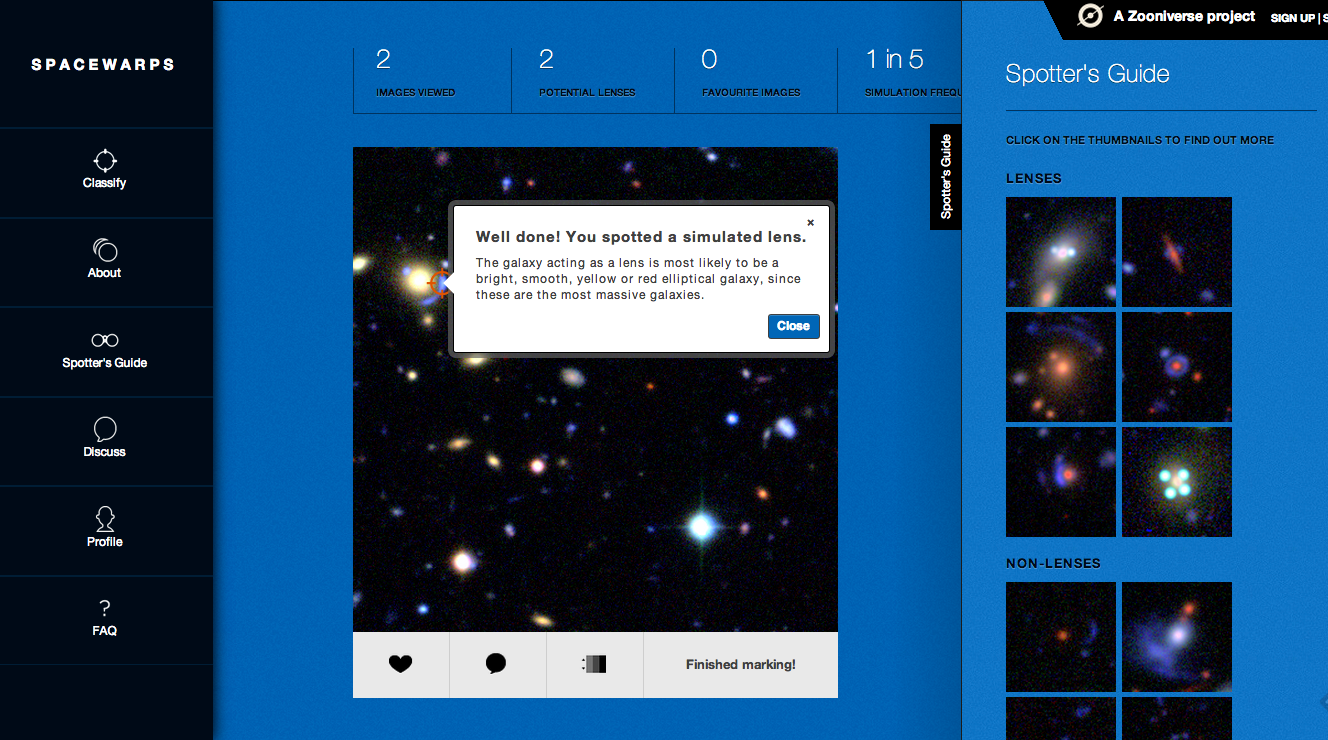
\includegraphics[width=0.9\linewidth]{sw-system-figs/sw-screengrab-marker+feedback.png}
% \caption{Screenshot of the \sw classification interface.}
% \label{fig:screenshot}
% \end{figure*}
% %%%%%%%%%%%%%%%%%%%%%%%%%%%%%%%%%%%%%%%

%%%%%%%%%%%%%%%%%%%%%%%%%%%%%%%%%%%%%%%%%%%%%%%%%%%%%%%%%%%%%%%%%%%%%%%%%%%%%%
%%  ACKNOWLEDGMENTS
%%%%%%%%%%%%%%%%%%%%%%%%%%%%%%%%%%%%%%%%%%%%%%%%%%%%%%%%%%%%%%%%%%%%%%%%%%%%%%

\section*{Acknowledgements}
 
We thank all \Ncollaboration members of the \sw community for their
contributions to the project so far. A complete list of collaborators is
provided at \texttt{http://spacewarps.org/\#/results/CFHTLS}.

We are also grateful to Stuart Lynn, Kelly Borden, Laura Whyte, Brooke Simmons,
David Hogg, Thomas Jennings, Layne  Wright, Cecile Faure, Jonathan Coles, Stuart
Lowe and Jean-Paul Kneib for many useful conversations about citizen science and
gravitational lens detection, and to the Dark Energy Survey and Pan-STARRS strong
lensing science teams for their suggestions and encouragement.

PJM was given support by the Royal Society, in the form of a research
fellowship, and by the U.S. Department of Energy under contract number DE-AC02-76SF00515.
%
AV acknowledges support from the Leverhulme Trust in the form of a research
fellowship.
%
The work of AM and SM was supported by World Premier International Research
Center Initiative (WPI Initiative), MEXT, Japan. The work of AM was also supported in
part by National Science Foundation Grant No. PHYS-1066293 and the hospitality
of the Aspen Center for Physics.
%
% Zooniverse / Sloan Foundation.
%
% Other authors.
PJM and ES thank the Institute of Astronomy and Astrophysics, Academia Sinica
(ASIAA) and Taiwan's Ministry of Science and Technology (MOST) for their
financial support of the workshop ``Citizen Science in Astronomy'' in March
2014, at which some parts of the SWAP analysis was developed.

The \sw project is open source.
The web app was developed at \texttt{https://github.com/Zooniverse/Lens-Zoo}, and was supported by a grant from the Alfred P. Sloan Foundation, 
while the SWAP analysis software was developed at
\texttt{https://github.com/drphilmarshall/SpaceWarps}.

The CFHTLS data used in this work are based on observations obtained with
MegaPrime/MegaCam, a joint project of CFHT and CEA/IRFU, at the
Canada-France-Hawaii Telescope (CFHT) which is operated by the National Research
Council (NRC) of Canada, the Institut National des Science de l'Univers of the
Centre National de la Recherche Scientifique (CNRS) of France, and the
University of Hawaii. This work is based in part on data products produced at
Terapix available at the Canadian Astronomy Data Centre as part of the
Canada-France-Hawaii Telescope Legacy Survey, a collaborative project of NRC and
CNRS.


%%%%%%%%%%%%%%%%%%%%%%%%%%%%%%%%%%%%%%%%%%%%%%%%%%%%%%%%%%%%%%%%%%%%%%%%%%%%%%
%  APPENDICES
%%%%%%%%%%%%%%%%%%%%%%%%%%%%%%%%%%%%%%%%%%%%%%%%%%%%%%%%%%%%%%%%%%%%%%%%%%%%%%

\appendix

%%%%%%%%%%%%%%%%%%%%%%%%%%%%%%%%%%%%%%%%%%%%%%%%%%%%%%%%%%%%%%%%%%%%%%%%%%%%%%

\section{Probabilistic Classification Analysis}
\label{appendix:swap}

Our aim is to enable the construction of a sample of good lens candidates.
Since we aspire to making logical  decisions, we define a  ``good candidate''
as one which has a high posterior probability of being a lens, given the data:
$\pr(\LENS|\data)$. Our problem is to approximate this probability. The data~$\data$
in our case are the pixel values of a colour image. However, we can greatly
compress these complex, noisy sets of data by asking each volunteer what they
think about them. A complete  classification in \sw consists of a set of
Marker positions, or none at all. The null set encodes the statement from
the volunteer that the image in question is $\saidNOT$ a lens, while the
placement of any  Markers indicates that the volunteer considers this image to
contain a $\saidLENS$.  We simplify the problem by only using the Marker
positions to assess whether the volunteer  correctly assigned the
classification $\saidLENS$ or $\saidNOT$ after viewing (blindly) a member of
the training set of subjects. 

How should we model these compressed data? The circumstances of each
classification are quite complex, as are the human classifiers in general: the
volunteers learn more about the problem as they go, but also inevitably make
occasional mistakes (perhaps because a lens is difficult to see, or they
became distracted during the task). To cope with this uncertainty, we assign a
simple software {\it agent} to partner each volunteer. The agent's task is to
interpret their volunteer's classification data as best it can, using a model
that makes a number of necessary approximations. These interpretations will
then include uncertainty arising as a result of the volunteer's efforts and
also the agent's approximations, but they will have two important redeeming
features. First, the interpretations will be quantitative (where before they
were qualititative),  and thus will be useful in decision-making. Second, the
agent will be able to predict, using its model, the probability of a test
subject being a $\LENS$, given both its volunteer's classification, and its
volunteer's experience. In this appendix we describe how these agents work,
and other aspects of the \sw analysis pipeline (SWAP).


\subsection{Agents and their Confusion Matrices}
\label{appendix:swap:probabilities}

Each agent assumes that the probability of a volunteer recognising any given
simulated lens as a lens is some number, $\pr(\saidLENS|\LENS,\training)$, that
depends only on what the volunteer is currently looking at, and all the
previous training subjects they have seen (and not on what type of lens it is,
how faint it is, what time it is, \etc). Likewise, it also assumes that the
probability of a volunteer recognising any given dud image as a dud is some
other number, $\pr(\saidNOT|\NOT,\training)$, that also depends only on what the volunteer is currently looking at, and all the
previous training subjects they have seen. These two probabilities define a 
2 by 2 ``confusion matrix,'' which the agent updates, every time a
volunteer classifies a training subject, using the following 
very simple estimate:
\be
  \pr(``X"|X,\training) \approx \frac{N_{``X"}}{N_X}.
  \label{eq:app:fraction}
\ee
Here, $X$ stands for the true classification of the subject, \ie either
$\LENS$ or $\NOT$, while $``X''$ is the corresponding classification
made by the volunteer on viewing the subject. $N_X$ is the number of
lenses the volunteer has been shown, while $N_{``X"}$ is the number of 
times the volunteer got their classifications of this type of training subject
right. $\training$ stands for all
$N_{\LENS} + N_{\NOT}$ training data that the agent has heard about to
date. 

The full confusion matrix of the $k^{\rm th}$ volunteer's agent is therefore:
\begin{align}
  \CM^k &= 
  \begin{bmatrix}
    \pr(\saidLENS|\NOT,\trainingk) & \pr(\saidLENS|\LENS,\trainingk) \\
    \pr(\saidNOT |\NOT,\trainingk) & \pr(\saidNOT |\LENS,\trainingk)
  \end{bmatrix}, \notag \\
        &=
  \begin{bmatrix}
    \CM_{LN} & \CM_{LL} \\
    \CM_{NN} & \CM_{NL}
  \end{bmatrix}^k.
  \label{eq:confmat}
\end{align}
Note that these probabilities are normalized, such that
$\pr(\saidNOT |\NOT) = 1 - \pr(\saidLENS|\NOT)$.

Now, when this volunteer views a test subject, 
it is this confusion matrix that will allow their agent to update the
probability of that test subject being a $\LENS$. Let us suppose that
this subject has never been seen before: the agent assigns a 
prior probability that it is (or contains) a lens is 
\be
  \pr(\LENS) = p_0
\ee
where we have to assign a value for $p_0$. In the CFHTLS, we might expect
something like 100 lenses in 430,000 images, so $p_0 = 2\times10^{-4}$
is a reasonable estimate. The volunteer then makes a classification $C_k$ 
($= \saidLENS$ or $\saidNOT$).
We can apply Bayes' Theorem to derive how the agent should
update this prior probability into a posterior one using this new information:
\begin{align}
  \label{eq:app:first}
  & \pr(\LENS|C_k,\trainingk) = \\
  & \frac{\pr(C_k|\LENS,\trainingk)\cdot\pr(\LENS)}
{\left[ \pr(C_k|\LENS,\trainingk)\cdot\pr(\LENS) + \pr(C_k|\NOT,\trainingk)\cdot\pr(\NOT) \right]},
  \notag
\end{align}
which can be evaluated numerically using the elements of the confusion
matrix. 

\subsection{Examples}
\label{appendix:swap:examples}

Suppose we have a volunteer who is always right about the true
nature of a training subject. 
Their agent's confusion matrix would be
\be
  \CM^{\rm perfect} = 
  \begin{bmatrix}
    0.0 & 1.0 \\
    1.0 & 0.0
  \end{bmatrix}.
\ee
On being given a fresh subject that actually is a $\LENS$, this hypothetical
volunteer would submit $C = \saidLENS$.  Their agent would then calculate the
posterior probability for the subject being a $LENS$ to be
\begin{align}
  \pr(\LENS|\saidLENS,\trainingk) &= \frac{1.0 \cdot p_0}
           {\left[ 1.0\cdot p_0 + 0.0\cdot(1 - p_0) \right]}
   &= 1.0,
\end{align}
as we might expect for such a {\it perfect} classifier.  Meanwhile, a
hypothetical volunteer who (for some reason) wilfully always submits the wrong
classification would have an agent with the column-swapped confusion matrix
\be
  \CM^{\rm obtuse} = 
  \begin{bmatrix}
    1.0 & 0.0 \\
    0.0 & 1.0
  \end{bmatrix},
\ee
and would submit $C = \saidNOT$ for this subject. However, such a volunteer
would nevertheless be submitting useful information, since given the above
confusion matrix, their agent would calculate
\begin{align}
  \pr(\LENS|\saidNOT,T_k) &= \frac{1.0 \cdot p_0}
           {\left[ 1.0\cdot p_0 + 0.0\cdot(1 - p_0) \right]}
   &= 1.0.
\end{align}
{\it Obtuse} classifiers turn out to be as helpful as {\it perfect} ones.


\subsection{Online SWAP: Updating the Subject Probabilities}
\label{appendix:swap:examples}

Suppose the $k+1^{\rm th}$ volunteer now submits a classification, on the same
subject just classified by the $k^{\rm th}$ volunteer. We can generalise
\Eref{eq:app:first} by replacing the prior probability with the current
posterior probability:
\begin{align}
  \label{eq:app:update}
  \pr(\LENS & |C_{k+1},\training_{k+1},\data) = \\
  & \frac{1}{Z} \pr(C_{k+1}|\LENS,\training_{k+1}) \cdot \pr(\LENS|\data) \\ \notag
{\rm where}\;\; Z = & \pr(C_{k+1}|\LENS,\training_{k+1})\cdot\pr(\LENS|\data) \\ \notag
      & + \pr(C_{k+1}|\NOT,\training_{k+1})\cdot\pr(\NOT|\data), \notag
\end{align}
and $\data = \{C_k,\trainingk\}$ is the set of all previous
classifications, and the set of training subjects seen by each of those
volunteers.
$\pr(\LENS|\data)$ is the fundamental property of each test subject that
we are trying to infer. We track $\pr(\LENS|\data)$ as a function of time,
and by comparing it to a lower or upper thresholds, make decisions about
whether to retire the subject from the classification interface or
promote it in \Talk, respectively.


\subsection{Information Gain per Classification, Agent ``Skill'' and ``Contribution''}
\label{appendix:swap:examples}

With an agent's confusion matrix in hand we can compute the
\emph{information} generated in any given classification. This will
depend on the confusion matrix elements (\Eref{eq:confmat}) but also on
the probability of the subject being classified containing a lens. The
quantity of interest is the relative entropy, or Kullback-Leiber
divergence, between the prior and
posterior probabilities for the possible truths $T$
given the submitted classification $C$:
\begin{align}
\information =& \sum_T \pr(T|C) \log_2 \frac{\pr(T|C)}{\pr(T)}     \notag \\
             =&    \pr(\LENS|C) \log_2 \frac{\pr(C|\LENS)}{\pr(C)} \notag \\
             +&    \pr(\NOT|C)  \log_2 \frac{\pr(C|\NOT)}{\pr(C)},
\end{align}
where, as above, $C$ can take the values $\saidLENS$ or $\saidNOT$. 
Substituting for the posterior probabilities using \Eref{eq:app:first} we get
an expression that just depends on the elements of the 
confusion matrix $\CM$ and the pre-classification subject lens
probability $\pr(\LENS) = p$:
\begin{align}
\information =    &     p \frac{\CM_{CL}}{p_c} \log_2 \frac{\CM_{CL}}{p_c}  \notag \\
                  & +(1-p)\frac{\CM_{CN}}{p_c} \log_2 \frac{\CM_{CN}}{p_c},
  \label{eq:app:infogain}
\end{align}
where the common denominator $p_c = p\CM_{CL} + (1-p)\CM_{CN}$. This
expression has many interesting features.  If $p$ is either zero or one,
$\information(C) = 0$  regardless of the value of $C$ or the values of
the confusion matrix elements: if we know the subject's status with
certainty, additional classifications supply no new information. If we
set $p$ to be the prior probability, \Eref{eq:app:infogain} tells us how
much information is generated by classifying it all the way to $p = 1$
(which a perfect classifier, with $\CM_{LL} = \CM_{NN} = 1$, can do in a
single classification). For a prior probability of $2\times 10^{-4}$, 
12.3 bits are generated in such a ``detection.''  Conversely, only
0.0003 bits are generated during the rejection of a subject with the
same prior: we are already fairly sure that each subject does not
contain a lens! Imperfect classifiers (with $\CM_{LL}$ and $\CM_{NN}$
both less than 1)  generate less than these maximum amounts of
information each classification; the only classifiers that generate zero
information are those that have $\CM_{LL} = 1 - \CM_{NN}$ (or
equivalently, $\CM_{CL} = \CM_{CN}$ for all values of $C$). We might
label such classifiers as ``random'', since they are as likely to
classify a subject as a $\saidLENS$ no matter the true content of that
subject. 

\Eref{eq:app:infogain} suggests a useful information theoretical 
definition of the classifier skill  perceived by the agent. At a fixed
value of $p$, we can take the expectation value of the information gain
$\information$ over  the possible classifications that could be made:
\begin{align}
\langle\information\rangle   =& \sum_C \sum_T \pr(T|C) \pr(C) \log_2 \frac{\pr(T|C)}{\pr(T)} \notag \\ 
         =& - \sum_T \pr(T) \log_2 \pr(T) \notag \\ 
          & + \sum_C \pr(C) \sum_T \pr(T|C) \log_2 \pr(T|C) \notag \\ 
         =&         p  \left[ \mathcal{S}(\CM_{LL}) + \mathcal{S}(1-\CM_{LL}) \right] \notag \\
          &     +(1-p) \left[ \mathcal{S}(\CM_{NN}) + \mathcal{S}(1-\CM_{NN}) \right] \notag \\
          & - \mathcal{S}\left[ p    \CM_{LL}       + (1-p)(1-\CM_{NN})     \right] \notag \\
          & - \mathcal{S}\left[ p (1-\CM_{LL})      + (1-p)   \CM_{NN}      \right] 
\end{align}
where $\mathcal{S}(x) = x \log_2{x}$. If we choose to
evaluate $\langle\information\rangle$ at $p = 0.5$, the result has some
useful properties. While random classifiers presented with  $p = 0.5$
subjects have $\skill = 0.0$  as expected, perfect classifiers appear to
the agents to have  $\skill = 1.0$. This suggests that  $\skill$, the
amount of information we expect to  gain when a classifier is presented
with a 50-50 subject, is a reasonable quantification of 
\emph{normalised skill}. A consequence of this choice is that the
integrated skill (over all agents' histories) should come out to be
approximately 
equal to the number of subjects in the survey, when the search is
``complete'' (and all subjects are fully classified). Therefore, a
particular agent's integrated skill is a reasonable 
measure of that classifier's
\emph{contribution} to the lens search.

We conservatively initialize both elements of each  agent's confusion
matrix to be $\CM^0_{LL} = \CM^0_{NN} = 0.5$, that of a maximally ambivalent  random classifier, so
that all agents start with zero skill. While  this makes no allowance
for volunteers that actually do have previous experience of what
gravitational lenses look like, we might expect it to help mitigate
against false positives. Anyone who classifies more than one image (by
progressing beyond the tutorial) makes a non-zero information
contribution to the project.

The total information generated during the CFHTLS project is shown in
\Tref{tab:crowd:contributions}. Interpreting these numbers is not easy, but we
might do the following. Dividing this by the amount of information it takes to
classify a \sw subject all the way to the detection threshold (lens
probability 0.95), and then multiplying by the survey inefficiency gives us a
very rough estimate for the effective number of detections corresponding to
the crowd's contribution: these are 2830 and 25 bits for stages 1 and 2
respectively.  These figures are close to the numbers of detections given in
column 7 of the table.  
% The uncertainty in the interpretation of the total
% information generated provides some justification for our focus on the
% expected information gain as a measure of volunteer contribution.


\subsection{Uncertainty in the Agent Confusion Matrices}
\label{appendix:swap:uncertainty}

Finally, the confusion matrix obtained from the application of
\Eref{eq:app:fraction} has some inherent noise which reduces as the
number of training subjects classified by the agent's volunteer
increases. For simplicity, the discussion has thus far assumed the case
when the confusion matrix is known perfectly; in practice, we allow for
uncertainty in the agent confusion matrices by averaging over a small
number of samples drawn from Binomial distributions characterised by the
matrix elements $\pr(C_k|\LENS,\trainingk)$ and  $\pr(C_k|\NOT,\trainingk)$. The
associated standard deviation in the estimated subject probability
provides an error bar for this quantity.

% For ease of notation, we will denote $\pr(C_k|\LENS,T_k)\equiv p_L$ and
% $\pr(C_k|\NOT,T_k)\equiv p_N$. In reality, there is a probability distribution
% for both $p_L$ and $p_N$. Let $p_0$ be the prior probability of the subject
% being a lens. Then the posterior probability, $p_0'$ of the subject being a
% lens after the classification $C_k$ is
% \be
%   \label{eq:app:sec}
% p_0' = \frac{p_L p_0}{\left[ p_L p_0 + p_N (1- p_0) \right]},
% \ee
% The posterior probability distribution $p_0'$ can be obtained by marginalizing
% over the probability distributions of $p_L$, $p_N$ and the prior probability
% distribution $p_0$ such that,
% \be
% P(p_0') = \int p_0' P(p_L) P(p_N) P(p_0) dp_L dp_N dp_0\,.
% \ee
% This marginalization is not analytically tractable. Therefore, we have
% implemented the following Monte-Carlo solution for this problem.
% 

%Finally, we also need to update the confusion matrix of an agent and obtain the
%variance on each element of the matrix, once a training subject has been
%classified. We would like to derive the posterior probability of the
%probability elements $p_1$ and $p_2$ given their prior probabilities. For this
%purpose, we can again make use of Bayes' theorem,
%\begin{equation}
%P(p_x'|N_{"X"},N_X,T) = \frac{P(N_{``X"}|p_x',N_X,T) P(p_x'|N_X,T)}{\sum_{N_{``X"}} P(N_{``X"}|p_x',N_X,T) P(p_x'|N_X,T)}
%\end{equation}
%Here, $P(N_{``X"}|p_x',N_X,T)$ is a binomial distribution, although this is not
%true strictly speaking given that our agents are learning and the values of the
%confusion matrix are moving. Modelling the learning curve of our users is yet
%another complicated extension we could think about.


\subsection{Offline SWAP}
\label{appendix:swap:offline}

The probabilistic model described above does not need to be implemented as an
online inference. Indeed, it might be more appropriate to perform the inference
of all Agent confusion matrix elements and Subject probabilities
simultaneously, so that the early classifications are not effectively
downweighted as a result of the Agent's ignorance. It might also be that this
ignorance builds in some conservatism to the system, reducing the noise due
the early classifications if they are unreliable. In the joint analysis, the
basic assumption that is built into the Agents, that their volunteers
have innate and unchanging talent for lens spotting parameterised by two 
constant confusion matrix elements which simply need to be inferred given the
data, is implemented in full. The effect is that of applying the time-averaged
confusion matrices, rather than one that evolves as the Agents (and in the
real world, the volunteers) learn. 

The mathematics of the offline inference are presented elsewhere (in
preparation). Here we briefly note that we maximize the joint posterior
probability distribution for all the model parameters (some 66,000 confusion
matrix elements and 430,000 subject probabilities) with a simple
expectation-maximisation algorithm. This procedure takes approximately the
same CPU time as the stage 2 online analysis, because no matrix inversions are
required in the algorithm. The algorithm scales well and is actually faster
than the online analysis with the larger stage 1 dataset. The
expectation-maximisation algorithm is robust to initial starting parameters
in, e.g., initial Agent confusion matrix elements and Subject probabilities.
The plots in \Sref{sec:results:sample} show the difference in performance
between the online and offline analyses. 


%%%%%%%%%%%%%%%%%%%%%%%%%%%%%%%%%%%%%%%%%%%%%%%%%%%%%%%%%%%%%%%%%%%%%%%%%%%%%%
%  REFERENCES
%%%%%%%%%%%%%%%%%%%%%%%%%%%%%%%%%%%%%%%%%%%%%%%%%%%%%%%%%%%%%%%%%%%%%%%%%%%%%%

% MNRAS does not use bibtex, input .bbl file instead. 
% Generate this in the makefile using bubble script in scriptutils:

% bubble -f paper-lcr.tex references.bib 
% \input{paper-lcr.bbl}

\bibliographystyle{apj}
\bibliography{references}


%%%%%%%%%%%%%%%%%%%%%%%%%%%%%%%%%%%%%%%%%%%%%%%%%%%%%%%%%%%%%%%%%%%%%%%%%%%%%%

\label{lastpage}
\bsp

\end{document}

%%%%%%%%%%%%%%%%%%%%%%%%%%%%%%%%%%%%%%%%%%%%%%%%%%%%%%%%%%%%%%%%%%%%%%%%%%%%%%
